\documentclass[a4paper,12pt]{article}
%\documentclass[fleqn]{article}

% ---パッケージ---
\usepackage{amsmath,amssymb}    %数式用
\usepackage{tcolorbox}   %囲み枠用(tcolorboxに変更)
\usepackage{geometry}   %余白調節
\usepackage{tikz}  % ← 図を描くためのTikZパッケージ
\geometry{margin=25mm}  %余白を少し狭く
\usetikzlibrary{decorations.pathmorphing,patterns,positioning,arrows.meta} % バネ・壁の模様
\tikzset{
  block/.style = {draw, rectangle, minimum height=2em, minimum width=3em},
  sum/.style = {draw, circle, inner sep=0pt, minimum size=5mm},
  input/.style = {coordinate},
  output/.style = {coordinate}
}
\usetikzlibrary{calc}


% --- 日本語用パッケージ ---
\usepackage{luatexja}         % 日本語表示に必要
\usepackage{luatexja-fontspec} % フォント指定用

% --- フォント指定(Overleaf標準フォント)---
\setmainjfont{IPAexMincho}  % 明朝体
%\setmainjfont{IPAexGothic}  % ゴシック体にしたい場合

% --- tcolorbox の設定 ---
\tcbset{
    colframe=black,
    colback=white,         % 本文の背景(白)
    boxrule=0.8pt,
    arc=3pt,
    outer arc=3pt,
    boxsep=4pt,
    coltitle=black,
    colbacktitle=gray!20,  % タイトルの背景(グレー)
    fonttitle=\normalsize
}

\begin{document}

\begin{tcolorbox}[title={1. (4)
    \vspace{-6mm}
    \begin{center}
        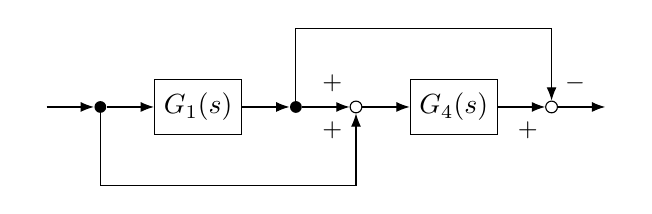
\begin{tikzpicture}[auto, node distance=0.4cm and 0.6cm, >=Latex]

        % --- 横並びノード(sum1 と branch2 の位置を交換) ---
        \node at (0,0) (input) {};
        \node[circle, fill=black, inner sep=1.5pt, right=of input] (branch2) {};     % ← 分岐2
        \node[block, right=of branch2] (G1) {$G_1(s)$};
        \node[circle, fill=black, inner sep=1.5pt, right=of G1] (branch1) {};        % 分岐1
        \node[circle, draw, inner sep=1.5pt, right=of branch1] (sum1) {};            % ← 合流1
        \node[block, right=of sum1] (G4) {$G_4(s)$};
        \node[circle, draw, inner sep=1.5pt, right=of G4] (sum2) {};                 % 合流2
        \node[right=of sum2] (output) {};
        
        % --- フィードバック座標 ---
        \coordinate (fb_down) at ($(branch2)+(0,-1.0)$);
        \coordinate (fb_up) at ($(branch1)+(0,1.0)$);
        
        % === 主系列 ===
        \draw[->] (input) -- (branch2);
        \draw[->] (branch2) -- (G1);
        \draw[->] (G1) -- (branch1);
        \draw[->] (branch1) -- (sum1);
        \draw[->] (sum1) -- (G4);
        \draw[->] (G4) -- (sum2);
        \draw[->] (sum2) -- (output);
        
        % === フィードバック経路 ===
        \draw[->] (branch2) |- (fb_down) -| (sum1);
        \draw[->] (branch1) |- (fb_up) -| (sum2);
        
        % --- 加算記号配置 ---
        \node at ($(sum1)+(-0.3,0.3)$) {\small $+$};
        \node at ($(sum1)+(-0.3,-0.3)$) {\small $+$};
        \node at ($(sum2)+(-0.3,-0.3)$) {\small $+$};
        \node at ($(sum2)+(0.3,0.3)$) {\small $-$};
        
        \end{tikzpicture}
    \end{center}  }]

    \begin{center}
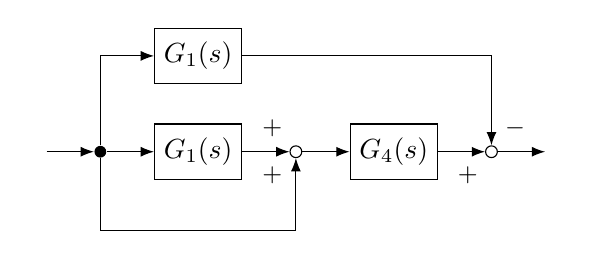
\begin{tikzpicture}[auto, node distance=0.4cm and 0.6cm, >=Latex]

% --- 横並びノード(分岐点を G1 の左に統一) ---
\node at (0,0) (input) {};
\node[circle, fill=black, inner sep=1.5pt, right=of input] (branch) {};           % 分岐点(統一)
\node[block, right=of branch] (G1) {$G_1(s)$};
\node[circle, draw, inner sep=1.5pt, right=of G1] (sum1) {};                      % 合流1
\node[block, right=of sum1] (G4) {$G_4(s)$};
\node[circle, draw, inner sep=1.5pt, right=of G4] (sum2) {};                      % 合流2
\node[right=of sum2] (output) {};

% --- 上ルートの追加ノード G₁(s) ---
\node[block, above=0.5cm of G1] (G1top) {$G_1(s)$};

% --- フィードバック座標(両方 branch 起点) ---
\coordinate (fb_down) at ($(branch)+(0,-1.0)$);
\coordinate (fb_up) at ($(branch)+(0,1.0)$);

% === 主系列 ===
\draw[->] (input) -- (branch);
\draw[->] (branch) -- (G1);
\draw[->] (G1) -- (sum1);
\draw[->] (sum1) -- (G4);
\draw[->] (G4) -- (sum2);
\draw[->] (sum2) -- (output);

% === 上ルート(branch → G1top → sum2)===
\draw[->] (branch) |- (G1top.west);
\draw[->] (G1top.east) -| (sum2.north);

% === フィードバック経路(そのまま) ===
\draw[->] (branch) |- (fb_down) -| (sum1);

% --- 加算記号配置 ---
\node at ($(sum1)+(-0.3,0.3)$) {\small $+$};
\node at ($(sum1)+(-0.3,-0.3)$) {\small $+$};
\node at ($(sum2)+(-0.3,-0.3)$) {\small $+$};
\node at ($(sum2)+(0.3,0.3)$) {\small $-$};

\end{tikzpicture}



    \vspace{2mm}
        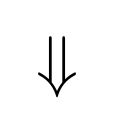
\begin{tikzpicture}
        \node {\Huge$\Downarrow$};
        \end{tikzpicture}
    \vspace{2mm}

    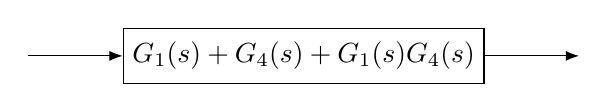
\begin{tikzpicture}[auto, node distance=2.0cm and 1.2cm, >=Latex]

    % --- 合成済みノード構成(完全伝達関数) ---
    \node[input] (input) {};
    \node[block, right=of input] (Gfinal) 
        {$ G_1(s) + G_4(s) + G_1(s)G_4(s)$};
    \node[output, right=of Gfinal] (output) {};

    % --- 線描画 ---
    \draw[->] (input) -- (Gfinal);
    \draw[->] (Gfinal) -- (output);

    \end{tikzpicture}

    \end{center}
\vspace{-4mm}
よって、システム全体の伝達関数\(G_{All}(s)\)は
\vspace{-2mm}
\[
G_{All}(s) = G_1(s) + G_4(s) + G_1(s)G_4(s)
\]
\end{tcolorbox}



\end{document}